\chapter{Review of the Literature}
\hl{Review of the spectrum of learning methods from reinforcement learning and adaptive control. With a focus on the reinforcement learning methods that can be applied in continuous state-action spaces. Really emphasising the fact that incorporating known information is novel.}

\section{Background}
Control theory is a discipline concerned with the behaviour of dynamical systems that can be specified by their inputs, states and outputs. This specification of dynamic system can include anything from aircraft to the stock market. The aim of control is to apply inputs to a system such that a desired output response is achieved. This is most often achieved using feedback, where the system outputs are available to the controller so that a mapping from outputs to inputs can be determined. One of the fundamental assumptions of control theory in general is that a mathematical model of the system is available that describes its dynamic behaviour to a reasonable degree of accuracy. This model is then used as though it was the real system to design feedback controllers.

An important area of control is how to design feedback control policies for unknown systems where control policies must be learned through interaction with the actual system. This problem has been the subject of Adaptive Control for many years. However, it has also been the subject of Reinforcement Learning. This is a framework born out of the Artificial Intelligence community and tackles the problem of learning a policy that is optimal with respect to some cost function given little or no prior knowledge about the system or environment. Originally these reinforcement learning methods were designed for systems with discrete state and input spaces, but recent advances have allowed algorithms for continuous systems to be defined.

A general framework for the problem of learning a discrete-time feedback control policy for an unknown system is shown in Figure~\ref{figs:learnframe}. It describes the full stochastic scenario where the systems unknown transition dynamics are governed by $p_f(X'|\bx,\bu), p_h(Y|\bx)$ where $\bx, \bu$ are the current state and input and $X', Y$ are the next state and output described by random variables. Note that a random variable is denoted using an upper case letter and a particular instance of this random variable is denoted in lower case. The scalar $c$ is some cost signal which encodes the goal of the control task required of the stochastic policy $\pi$ with tuneable parameters $\bpsi$.

Although references have been made in the literature to the similarity of these two learning paradigms there has been no formal unification under a single framework. This is a striking gap. The merging of the fields would be an important step as it would lead to the investigation of whether the incorporation of concepts from one approach into the other could yield improved performance. Further, it would be advantageous to discover whether classes of control problems can be determined for which one approach would be more efficacious or preferable. This report will begin with a formal review of the literature and methods of both adaptive control and reinforcement learning.

\begin{figure}
\centering
% Define block styles
\tikzstyle{block} = [thick, rectangle, draw, text width=7em, text centered, rounded corners, minimum height=4em, fill=black!15]
\tikzstyle{bloc2k} = [thick,rectangle, draw, text width=10em, text centered, rounded corners, minimum height=5em, fill=black!25]
\tikzstyle{sum} = [thick,circle, draw, minimum height=.5cm]
\tikzstyle{line} = [draw, -latex]
\tikzstyle{dot} = [circle, draw, fill=black, inner sep=1pt]
\begin{tikzpicture}[rounded corners]

	\node at(5,-2.8) [block](adapt){\textbf{Adaptation}};	
        \path[line] (adapt.south) |- (-1.2,-4) -- (-1.2,-1.2) -- (1.2,1.2);

	% Place nodes
	\node at(0,0) [block](pol){\textbf{Policy} \\[0.1cm]$\bu = \bpi(\bx,\br)$};
	\node at(5,0) [bloc2k](sys){\textbf{System} \\[0.1cm]$\bx_+ = \bff(\bx,\bu)$};
	
	\node at(2.2,0)[dot](dot1){};
	\node at(7.8,0)[dot](dot2){};
	
	% Draw arrows
	\path[line] (pol.east) -- (sys.west);
        \path[line] (sys.east) -- (dot2) |- (adapt.east);
        \path[line] (dot2.east) -- ([xshift=1cm] dot2.east);
        \path[line] (dot1) |- (adapt.west);
        \path[line] (dot2) |- ([xshift=-1cm,yshift=1.8cm] pol.west) |- ([yshift=0.4cm]pol.west);
        \path[line] ([xshift=-1cm,yshift=-0.4cm] pol.west) -- ([yshift=-0.4cm]pol.west);
        \path[line] (sys.south) -- (adapt.north);

	% Labels
	\node at (-2,-0.2) {$\br$};
        \node at (-2,0.6) {$\bx$};
        \node at (8.3,0.3) {$\bx$};
        \node at (2.2,0.3) {$\bu$};
        \node at (-0.8,-3.6) {$\bpsi$};
        \node at ([xshift=0.7cm,yshift=-0.5cm] sys.south) {$c(\bx,\bu)$};

\end{tikzpicture}

\caption{The general framework for learning a parameterised discrete-time state-feedback control policy $\pi$ to map the system state $\bx$ and some reference signal $\br$ to a distribution over the input $\bu$. The adaptation block can be carried out online or offline and can make use of some scalar cost signal $c$ which defines the desired task or system performance. The deterministic case simply reduces the probability distributions to delta functions and therefore direct mappings.}
\label{figs:learnframe}
\end{figure}


\section{Reinforcement Learning} %%%%%%%%%%%%%%%%%%%%%%%%%%%%%%%%%%%%
\subsection{Introduction}
Reinforcement learning is a field that was born, in the form that can be seen today, during the early 1980s. It was formed by the combination of two main threads of independent research. One thread was research carried out in optimal control and solutions involving the use of dynamic programming based methods. Although this did not involve learning as such, the algorithms gradually reach the correct solution through successive approximations so were considered among the other reinforcement learning methods. The other was was research in learning by trial and error which started in the psychology of animal learning and led to Monte-Carlo methods for learning\footnote{Not to be confused with Monte-Carlo statistical methods in general.}. Concepts from each of these threads were then combined to form a what is known as reinforcement learning today, a cornerstone of which were the Temporal Difference (TD) methods. One of the most famous successes of early TD methods came in the development of a world-class computer backgammon player in \cite{Tes92,Tes95}. Good reviews of the early literature in the field of reinforcement learning and the basic concepts can be found in \cite{SuBa98}, \cite{KLM96} and \cite{BerTs96} for a more in depth analysis.


\subsection{Markov Decision Process Framework}
Reinforcement Learning (RL) algorithms assume the framework of a Markov Decision Process (MDP). MDPs are discrete-time dynamical systems where the next state is dependant only on the current state $\bx_k \in \cX \subset \RR^n$ and action $\bu_k \in \cU \subset \RR^m$, a property known as the Markov property. The system is in some initial state $\bx_0 \sim p_0(X_0)$ and at any state $\bx_k$ the agent will use draw an action from the policy distribution $\bu_k \sim \pi(U_k|\bx_k)\in\Pi$ (or $\pi(U_k|\bx_k,\bpsi)$ for a parameterised policy). The system will evolve to a new state according to the unknown transition dynamics $\bx_{k+1} \sim p_f(X_{k+1}|\bx_k,\bu_k)$ and will return a scalar cost signal $c_k \sim p_c(C_k|\bx_k,\bu_k) \in \RR$. The cost function will be assumed to be deterministic for the remainder of this thesis, $c_k = c(\bx_k,\bu_k)$.

A trajectory through the state-action space of an MDP is denoted $\btau = \{\bx_{0:H},\bu_{0:H}\} \in \mathcal{T} = (H+1)(\cX\times\cU)$ where $H$ is the task horizon. The probability of a trajectory being generated by a given policy is $P(\btau|\pi) = \pi(\bu_0|\bx_0) p_0(\bx_0)\prod_{k=1}^H \pi(\bu_k|\bx_k) p_f(\bx_{k}|\bu_{k-1},\bx_{k-1}) $. The cumulative cost $\rho(\btau)$ or return\footnote{Technically the negative return since we are dealing with costs not rewards.} for some trajectory $\btau$ is defined as
\begin{equation}
\rho(\btau) = \sum^H_{k=0} a_kc_k,
\end{equation}
where $a_k$ is some time dependent weighting factor. Common examples are the \textit{discounted return} $a_k=\gamma^k$ where $\gamma \in (0,1]$ and the \textit{average return} $a_k = 1/H$. The general goal of reinforcement learning is to find a policy such that the expected return
\begin{align}
J(\pi) &= \EE_{\btau} \big[\rho(\btau) | \pi \big] = \int_{\mathcal{T}} \rho(\btau) P(\btau|\pi) \dd \btau,
\end{align}
is minimised. The notation $\EE_{\btau}[\cdot|\pi]$ denotes the expectation under trajectory $\btau$ given policy $\pi$ is applied. The policy that yields the minimum expected return is denoted $\pi^*$.

Important concepts in reinforcement learning and optimal control are that of the value function $V^\pi(\bx,k)$ and action-value function $Q^\pi(\bx,\bu,k)$. The value function is the expected return if policy $\pi$ is followed from state $\bx_k$. Similarly, the action-value function returns the expected return of taking action $\bu_k$ in state $\bx_k$ then choosing actions according to the policy $\pi$ thereafter. In mathematical terms 
\begin{align}
V^\pi(\bx,k) &= \EE_{\btau}\Bigg[ \sum^H_{l=k} a_lc_l \bigg|\bx_k=\bx,\pi \Bigg], \\
Q^\pi(\bx,\bu,k) &= \EE_{\btau}\Bigg[ \sum^H_{l=k} a_lc_l \bigg|\bx_k=\bx,\bu_k=\bu,\pi \Bigg].
\end{align}
In the infinite horizon case (as $H\rightarrow\infty$), these functions become time-invariant so are denoted $V^\pi(\bx)$ and $Q^\pi(\bx,\bu)$ respectively. Note that the expected return can be written in terms of the value function by averaging over all possible start states $\bx_0$, $J(\pi) = \int_{\cX} p(\bx_0)V^\pi(\bx_0,0)\dd\bx_0$.
The optimal value function is given by
\begin{equation}
V^*(\bx) = \min_{\pi \in \Pi} [V^\pi(\bx)],
\end{equation}
where an optimal policy is the argument to the minimal solution $\pi^*(\bx) = \arg\min_{\pi \in \Pi} V^\pi(\bx)$. The action-value function and value function are linked through the relationship $V^\pi(\bx) = \EE_{\bu} [Q^\pi(\bx,\bu)|\bx,\pi]$. Similarly, the optimal action-value function is related to the optimal value function through the relationship $V^*(\bx) = \min_{\bu \in \cU} [Q^*(\bx,\bu)]$.




\subsection{Dynamic Programming}
The dynamic programming paradigm of \cite{Bell57} is the framework that most reinforcement learning algorithms use to find an optimal policy. In order to introduce the concepts attention will be restricted to the infinite horizon ($T \rightarrow \infty$), discounted return ($a_k=\gamma^k$) case. It can be observed that the value function satisfies the Bellman (fixed-point) equation
\begin{equation}
V^\pi(\bx) =  \EE_{\bx',\bu} \Big[ c + \gamma V^\pi(\bx') \big|\bx,\pi \Big]
\end{equation}
where $c \sim p_c(C|\bx,\bu)$ and $\bx' \sim p_f(X'|\bx,\bu)$. The optimal value function satisfies the Bellman \textit{optimality} equation (otherwise known as the discrete-time Hamilton-Jacobi-Bellman (HJB) equation)
\begin{equation}
V^*(\bx) = \min_{\bu\in\cU} \EE_{\bx'} \Big[c + \gamma V^*(\bx') \big|\bx,\bu\Big].
\end{equation}
Under the assumption that the system dynamics are in fact known, two forward in time algorithms can be defined: Policy Iteration and Value Iteration. Each one iterates between \textit{evaluation} of the value function of a given policy and \textit{improvement} of the policy but making it ``greedy" with respect to the current value function.


%%
%\begin{wrapfigure}{r}{0.5 \textwidth}
\begin{figure}
\begin{center}
% Define block styles
\tikzstyle{block} = [thick, rectangle, draw, text width=3em, text centered, rounded corners, minimum height=3em, fill=black!15]
\tikzstyle{line} = [draw, -triangle 60]
\tikzstyle{dot} = [circle, draw, fill=black, inner sep=1pt]
\begin{tikzpicture}[rounded corners]

	% Place nodes
	\node at(-2,0) [block](pie){\Large $\pi$};
	\node at(2,0) [block](vee){\Large $V$};
	\node at(7,0) [block](pie0){\Large $\pi^*$};
	\node at(10,0) [block](vee0){\Large $V^*$};
	
	\path[line] (pie.north) |- ([yshift=0.8cm]vee.north) -- (vee.north);
	\path[line] (vee.south) |- ([yshift=-0.8cm]pie.south) -- (pie.south);
	\path[line] ([yshift=0.2cm]pie0.east) -- ([yshift=0.2cm]vee0.west);
	\path[line] ([yshift=-0.2cm]vee0.west) -- ([yshift=-0.2cm]pie0.east);
	
	\node at (4,0)[dot]{}; \node at (4.5,0)[dot]{}; \node at (5,0)[dot]{};
	
	\node at (0,1.7){\textbf{Evaluation}};
	\node at (0,1.1){$V \rightarrow V^\pi$};
	\node at (0,-1.1){\textbf{Improvement}};
	\node at (0,-1.7){$\pi\rightarrow\mathrm{greedy}(V)$};

\end{tikzpicture}

\end{center}
\caption{Generalised Policy Iteration}
\label{figs:GPI}
\end{figure}
%\end{wrapfigure}
%%

\textbf{Policy Iteration} \\[-0.3cm]
\hrule
Initialise procedure with some policy $\pi_0$. Iterate the following steps until convergence: 

\textbf{Evaluation:} Determine the value of policy $\pi_j$ by finding the value function $V_{j+1}$ that satisfies $V_{j+1}(\bx) = \EE_{\bx',\bu} \big[c + \gamma V_{j+1}(\bx') |\bx,\pi_j \big]$.

\textbf{Improvement:} Determine an improved policy $\pi_{j+1}$ by being greedy with respect to the value function $V_{j+1}$ using $\pi_{j+1}(\bx) = \arg\min_{\bu\in\cU} \EE_{\bx'} \big[ c + \gamma V_{j+1}(\bx')|\bx,\bu\big]$. \\[-0.1cm]
\hrule

\vspace{0.2cm}
\textbf{Value Iteration} \\[-0.3cm]
\hrule
Replace evaluation step in Policy Iteration with a truncation by setting $V_{j+1}(\bx) = \EE_{\bx',\bu} \big[c + \gamma V_{j}(\bx') |\bx,\pi_j\big]$ where $V_{j+1}$ has been replaced by $V_j$ on the right hand side. \\[-0.1cm]
\hrule
\vspace{0.2cm}


Both Policy Iteration and Value Iteration can be viewed under the Generalised Policy Iteration scheme of \cite{SuBa98} as displayed in Figure~\ref{figs:GPI} where evaluation and improvement steps are interleaved. In fact, all value function based schemes can be viewed under this framework.



Even if these algorithms were carried out using only data from interaction with the system, some a priori knowledge of the system dynamics is required in the improvement step, which is common to both algorithms. In order to find the minimal solution, the derivative with respect to the input $\bu$ is required which leads to the necessity of knowing the derivative $\partial\bx'/\partial\bu$ (the $B$ matrix if system is linear). This problem is alleviated in reinforcement learning algorithms through the use of the action-value function in place of the value function. 
The action-value function satisfies
\begin{equation}
Q^\pi(\bx,\bu) = \EE_{\bx',\bu'} \Big[ c + \gamma Q^\pi(\bx',\bu') \big|\bx,\bu,\pi \Big]. \label{eqn:Qfixed}
\end{equation}
The optimal action-value function satisfies
\begin{equation}
Q^*(\bx,\bu) = \EE_{\bx'} \Big[ c + \gamma \min_{\bu'\in\cU}\big[Q^*(\bx',\bu')\big] \big|\bx,\bu \Big].
\end{equation}
How these can be used as the basis of practical algorithms is the subject of the following section.


\subsection{Temporal Differences}
\subsubsection{Bootstrapping Methods}
Bootstrapping methods are based on estimating the Temporal Difference (TD)-error which will be defined below. The term `bootstrapping' pertains to the idea concept that estimates of parameters are based on estimates of other parameters. These methods are ways of evaluating or estimating the value function of a given policy $V^\pi$ (not considered further, since knowledge of the system dynamics is required to find a policy), the action-value function $Q^\pi$ ($\SARSA$) or the optimal action-value function $Q^*$ directly (\Q-learning). They have enjoyed much empirical success in the discrete state-space domain, including learning how to play backgammon \cite{Tes92,Tes95} and chess \cite{BTW00}. These methods utilise the TD-error, or Bellman error, as part of a stochastic gradient descent algorithm. In most applications it is necessary to maintain a parametric approximation of these functions, denoted by $\hat V_{\bth}$ and $\hat Q_{\bth}$ where $\bth$ is the vector of free parameters. Borrowing from the survey paper of \cite{GP10b} the following cost functions are minimised
\begin{align}
J_{Q^{\pi}}(\bth) &= \parallel Q^\pi - \hat Q_{\bth} \parallel^2, \label{eqn:JQcost1} \\
J_{Q^*}(\bth) &= \parallel Q^* - \hat Q_{\bth} \parallel^2 , \label{eqn:JQcost2}
\end{align}
for $\SARSA$ and \Q-learning respectively. Finding the optimal setting for the parameters $\bth$ is achieved using a stochastic gradient descent where the parameters are adjusted according to an approximation of the gradient of the cost function. Given an observation of a transition $(\bx,\bu,c,\bx',\bu')$ for $\SARSA$ or $(\bx,\bu,c,\bx')$ for $\mathcal{Q}$-learning the update law is given by
\begin{equation}
\bth_i = \bth_{i-1} + \alpha_i \Big( \nabla_{\bth_{i-1}}\hat Q_{\bth}(\bx,\bu) \Big) \Delta_{i} ,
\end{equation}
where $\alpha_i$ is a learning rate that satisfies the classical stochastic approximation criterion $\sum^\infty_{i=1} \alpha_i = \infty, \sum^\infty_{i=1} \alpha_i^2 < \infty$ and the TD-error $\Delta_{i}$ is given by
\begin{align}
\Delta_{i} &=  c + \gamma \hat Q_{\bth_{i-1}}(\bx',\bu') - \hat Q_{\bth_{i-1}}(\bx,\bu), \\
\Delta_{i} &=  c + \gamma \min_{\bu' \in \cU}\hat Q_{\bth_{i-1}}(\bx',\bu') - \hat Q_{\bth_{i-1}}(\bx,\bu),
\end{align}
for $\SARSA$ and \Q-learning respectively. It should be noted that in approximating the action-value function (as in \SARSA) the agent must be following the policy $\pi$ in order to converge. This is known as an \textit{on-policy} method. A convergence proof of $\SARSA$ with linear function approximation in finite state-action space can be found in \cite{TV97}. \Q-learning was introduced for the discrete space, look-up table formulation, in the thesis by \cite{Wat89} with convergence proofs following in \cite{WD92}. It is an \textit{off-policy} method since it can follow an arbitrary policy (provided it explores sufficiently in the state-action space) but will converge to the optimal action-value function. The proof of convergence for both $\SARSA$ and \Q-learning with linear function approximation, continuous state space and finite action space followed much later in \cite{MMR09}.

\subsubsection{Fitted Q-Iteration}
An important extension of the standard \Q-learning algorithm was presented by \cite{EGW05} and seeks to combine the \Q-learning principle with supervised learning methods to form a batch algorithm.

Compared with MPC in \cite{EGCW09}.


\subsubsection{Residual Methods}
As opposed to minimising the cost functions given by (\ref{eqn:JQcost1}) and (\ref{eqn:JQcost2}) one could minimise the error obtained by forcing the function approximation to satisfy the fixed point equation (\ref{eqn:Qfixed})
\begin{equation}
J(\bth) = \parallel \hat Q_{\bth} - (c + \gamma \hat Q_{\bth}) \parallel^2.
\end{equation}
This method does not lend itself to the stochastic gradient descent method outlined in the previous section because a penalty term arises which acts to favour smooth functions and hence gives a biased estimate of the optimal solution. However, least squares approaches to the this minimisation have worked well. For example Gaussian Process Temporal Differences (GPTD) of \cite{EMM03,EMM05} or Kalman Temporal Differences (KTD) of \cite{GPF09} (see \cite{GP10a} for a full derivation).



\subsubsection{Issues}
There are a few notable problems with the algorithms outlined in this section. The most important is that they do not scale well to continuous state-action spaces and problems of practical interest where it is unreasonable to search the entire state-action space (except the fitted Q-iteration algorithm). There is also the problem of reconstructing a useable or parameterised policy from the action-value function once it has been learned (a notable exception is when the system is affine and the cost is quadratic in the control actions).

One class of reinforcement learning algorithms that has been able to overcome these issues are policy-gradient algorithms and are the subject of the following section.







\subsection{Policy-Gradient Algorithms}
\subsubsection{Background}
The aim of policy-gradient algorithms is to directly adjust policy parameters $\bpsi$ by utilising an estimate of the gradient of the expected return with respect to the policy parameters $\nabla  J(\bpsi)$. Note that $\nabla = \nabla_{\bpsi}$ unless otherwise specified. Such algorithms are often referred to as \textit{Actor-Critic Methods} where the `critic' maintains the estimate of the action-value function which in turn informs the `actor' how to update its parameters. The actor-critic layout is shown in Figure~\ref{figs:actorcritic}. The policy parameters of the `actor' are updated in the direction of the negative gradient provided by the `critic' according to the adjustment law
\begin{equation}
\bpsi_{i+1} = \bpsi_{i} - \alpha_i \nabla J|_{\bpsi=\bpsi_i}
\end{equation}
where the learning rate $\alpha_i$ satisfies $\sum_{i=0}^{\infty} a_i = \infty$ and $\sum_{i=0}^{\infty} a_i^2 < \infty$. Since the policy $\pi$ is now fully characterised by its free parameters $\bpsi$ the expected return $J(\pi)$ can be written $J(\bpsi)$.

%%
\begin{figure}
\centering
% Define block styles
\tikzstyle{block} = [thick, rectangle, draw, text width=7em, text centered, rounded corners, minimum height=4em, fill=black!15]
\tikzstyle{bloc2k} = [thick,rectangle, draw, text width=10em, text centered, rounded corners, minimum height=5em, fill=black!25]
\tikzstyle{sum} = [thick,circle, draw, minimum height=.5cm]
\tikzstyle{line} = [draw, -latex']
\tikzstyle{dot} = [circle, draw, fill=black, inner sep=1pt]
\begin{tikzpicture}[rounded corners]

	\node at(5,-2.8) [block](adapt){\textbf{Critic} \\[0.1cm] $\bpsi \leftarrow \bpsi - \alpha \nabla J$};
        \path[line] (adapt.south) |- (-1.2,-4) -- (-1.2,-1.2) -- (1.2,1.2);

	% Place nodes
	\node at(0,0) [block](pol){\textbf{Actor} \\[0.1cm]$\pi(U|\bx,\br,\bpsi)$};
	\node at(5,0) [bloc2k](sys){\textbf{System} \\[0.1cm]$p_f(X'|\bx,\bu)$};
	
	\node at(2.2,0)[dot](dot1){};
	\node at(7.8,0)[dot](dot2){};
	
	% Draw arrows
	\path[line] (pol.east) -- (sys.west);
        \path[line] (sys.east) -- (dot2) |- (adapt.east);
        \path[line] (dot2.east) -- ([xshift=1cm] dot2.east);
        \path[line] (dot1) |- (adapt.west);
        
        \path[line] (dot2) |- ([xshift=-1cm,yshift=1.8cm] pol.west) |- (pol.west);
        \path[line] (sys.south) -- (adapt.north);

	% Labels
        \node at (-2,0.3) {$\bx$};
        \node at (8.3,0.3) {$\bx$};
        \node at (2.2,0.3) {$\bu$};
        \node at (-0.8,-3.6) {$\bpsi$};
        \node at ([xshift=1cm,yshift=-0.5cm] sys.south) {$p_c(C|\by,\bu)$};

\end{tikzpicture}

\caption{Layout of the actor-critic policy gradient scheme.}
\label{figs:actorcritic}
\end{figure}
%%

The problem is how to obtain a good estimate of the gradient. Two prominent approaches can be found in the literature: finite-difference and likelihood ratio methods. For an overview of these methods the reader is directed to the article by \cite{PS08}. Finite-difference methods can be dated back as far as the 1950s, originating in stochastic simulation community. They involve simply performing several roll-outs on the system using perturbed policy parameters $\bpsi+\Delta\bpsi$ and turning the gradient estimation into a regression problem. However, determining the size of $\Delta\bpsi$ requires good knowledge of the system and can be hard to tune without expert guidance. For this reason, these methods shall not be pursued further. Likelihood ratio methods are based on the \textit{likelihood ratio trick}.

\cite{Mun06} provides an alternative to the likelihood ratio method that is not subject to variance explosion at the discrete timesteps approach zero. This is a neat theoretical trick but it does not come with a practically implementable algorithm.

\subsubsection{The Likelihood Ratio Trick}
The gradient of the expected return can be written analytically as
\begin{align}
\nabla J(\bpsi) &= \int_{\cT} \rho(\btau) \nabla P(\btau|\pi) \dd \btau \\
&= \int_{\cT}  \rho(\btau) P(\btau|\pi)\nabla\log P(\btau|\pi) \dd \btau \\
&= \EE_{\btau} \Big[ \rho(\btau) \nabla\log P(\btau|\pi)  \big|\pi \Big].
\end{align}
This form is useful in two ways. The first is that it lends itself to sample based approximation given a set of trajectories sampled from the MDP using policy parameters $\bpsi$ Secondly, $\nabla \log P(\btau|\pi) = \sum_{k=0}^H \nabla \log \pi(\bu_k|\bx_k)$ which requires no knowledge of the system dynamics to calculate. Also, since the integral $\int_{\cT}b \nabla  P(\btau|\pi) \dd \btau = 0$ for an arbitrary constant $b$, the gradient can be written as
\begin{equation}
\nabla J(\bpsi) = \EE_{\btau} \Big[ (\rho(\btau) - b) \nabla \log P(\btau|\pi)  \big|\pi \Big].
\end{equation}
This is the basis of the episodic REINFORCE algorithm of \cite{Wil92}. Although $b$ has no effect on the mean of the gradient estimate it can have a huge effect on the variance of the estimate and can be chosen so as to minimise this variance. The optimal baseline was derived by \cite{PS08}. Improved algorithms were developed by \cite{SMSM00} and \cite{MT01} with the Policy Gradient Theorem and \cite{BB01} with GPOMDP. They make the intuitive observation that future actions are independent of past rewards. \cite{PS08} show from a trajectory based perspective these algorithms are in fact equivalent. We shall now look further at the Policy Gradient Theorem.

\subsubsection{The Policy Gradient Theorem}
For the infinite horizon, normalised ($\sum_{k=0}^\infty a_k=1$) case the expected return can be written in state-space form (see \cite{SMSM00})
\begin{equation}
J(\pi) = \int_{\cX} d^\pi(\bx) \int_{\cU} \pi(\bx|\bu) c(\bx,\bu) \dd \bu\dd\bx
\end{equation}
where $d^\pi(\bx) = \sum_{k=0}^\infty a_kp(\bx_k=\bx)$ is the weighted state distribution which is assumed to be independent of $\bx_0$ for all policies.

The \textit{Policy Gradient Theorem} (see Theorem 1, \cite{MT01} or Proposition 1, \cite{SMSM00} for the original derivations) states that for any MDP the following relationship holds 
\begin{equation}
\nabla  J(\bpsi) = \int_{\cX} d^\pi(\bx) \int_{\cU} \nabla  \pi(\bx|\bu) \Big( Q^\pi(\bx,\bu) - b^\pi(\bx) \Big) \dd\bu\dd\bx, \label{eqn:Jgrad}
\end{equation}
for an arbitrary baseline $b^\pi(\bx)$. It was further shown by \cite{MT01} and \cite{SMSM00} that the term $Q^\pi(\bx,\bu) - b^\pi(\bx)$ can be replaced by a \textit{compatible function approximation}
\begin{equation}
f^\pi_{\bth}(\bx,\bu) = \big(\nabla  \log \pi(\bu|\bx)\big)^\top \bth \equiv Q^\pi(\bx,\bu) - b^\pi(\bx),
\end{equation}
which does not affect the unbiasedness of the gradient estimate and is irrespective of the choice of baseline. Substituting this into the gradient equation (\ref{eqn:Jgrad}) gives the following
\begin{equation}
\nabla  J(\bpsi) = \int_{\cX} d^\pi(\bx) \mathbf{\hat G}_{\bth}(\bx) \dd\bx \; \bth = \mathbf{G}_{\bth} \bth,
\end{equation}
where the integral $\mathbf{\hat G}_{\bth}(\bx) = \int_{\cU} \pi(\bu|\bx)\nabla \log\pi(\bu|\bx)\nabla \log\pi(\bu|\bx)^\top \dd\bu$ can be evaluated analytically since $\pi(\bu|\bx)$ is specified by the user. However, evaluating $\mathbf{G}_{\bth}$ is still expensive since the stationary distribution $d^\pi(\bx)$ is unknown.

A major issue with the algorithms discussed so far tend to reduce exploration noise in the policy too quickly and therefore converge slowly on the optimal solution. \cite{Kak02} showed that this problem is a product of using the standard gradient metric but can be overcome through the use of the \textit{natural policy gradient}.


\subsubsection{The Natural Policy Gradient}
Rather than following the steepest direction in parameter space the natural gradient follows the steepest descent direction with respect to the Fisher information matrix $\mathbf{F}_{\bth}$
\begin{equation}
\tilde\nabla  J(\bpsi) = \mathbf{F}_{\bth}^{-1} \nabla  J(\bpsi).
\end{equation}
The method came out of the supervised learning community where \cite{Ama98} showed that the natural gradient is superior to the standard gradient method since it exploits the properties of Riemannian manifolds. It was first utilised in a reinforcement learning context by \cite{Kak02} who demonstrated improved performance over the standard method. But it was the contribution of \cite{PVS05} to show that the Fisher information matrix $\mathbf{F}_{\bth}$ is in fact identically equal to the matrix $\mathbf{G}_{\bth}$ derived in the previous section. Therefore, utilising natural policy gradients we have the very elegant result that
\begin{equation}
\tilde\nabla J(\bpsi) = \mathbf{F}_{\bth}^{-1} \mathbf{G}_{\bth} \bth = \bth.
\end{equation}
Therefore the only remaining issue is to estimate the parameter vector $\bth$ of the compatible function approximation.
It is important and interesting to note that $f^\pi_{\bth}(\bx,\bu)$ is mean zero with respect to the action distribution ($\int_{\cU} \pi(\bu|\bx) f^\pi_{\bth}(\bx,\bu) = \bth^\top \int_{\cU} \nabla\pi(\bu|\bx) =0$). Therefore it represents an \textit{advantage function} $A^\pi(\bx,\bu) = Q^\pi(\bx,\bu) - V^\pi(\bx)$ implying that the baseline $b^\pi(\bx)$ has implicitly been set to the value function. However, the advantage function cannot be estimated using TD-like bootstrapping methods without also maintaining an estimate of the value function $V^\pi(\bx)$ which can lead to problems if the function approximation scheme is chosen innappropriately.

This problem can be overcome with a couple of mild assumptions resulting in the Episodic Natural Actor-Critic algorithm of \cite{PVS05}. A Bellman-like equation in terms of the advantage function can be written as
\begin{equation}
\sum_{k=0}^H a_k A^\pi(\bx_k,\bu_k) = a_{H+1}V^\pi(\bx_k) + \sum_{k=0}^H a_k c(\bx_k,\bu_k) - V^\pi(\bx_0).
\end{equation}
Therefore, assuming a long task horizon $a_{H+1} \rightarrow 0$ (or $c(\bx_H,\bu_H)$ is the final cost) and a narrow start state distribution so that $V^\pi(\bx_0)$ can be approximated by a single scalar $J_0$, a simple regression problem results
\begin{equation}
\sum_{k=0}^H a_k \nabla\log\pi(\bx_k,\bu_k)^\top \bth + J_0 = \sum_{k=0}^H a_k c(\bx_k,\bu_k)
\end{equation}
with $\mathrm{dim}\bth +1$ unknowns. So for a deterministic system, only $\mathrm{dim}\bth +1$ rollouts are required to find the natural gradient using least-squares regression
\begin{equation}
\begin{bmatrix}\bth \\ J_0 \end{bmatrix} = (\bPh^\top \bPh)^{-1} \bPh^\top\bPsi,
\end{equation}
where $\bPh_i = [\sum_{k=0}^H a_k \nabla\log\pi(\bu_k|\bx_k)^\top,1]$ and $\bPsi_i = \sum_{k=0}^H a_kc(\bu_k,\bx_k)$.




\subsubsection{Model-Based Policy Gradients}
Now all the methods discussed so far have been model free in the sense that a model of the actual system has not been required or estimated. The main reason for avoiding model-based methods is that most algorithms substitute the learned model in place of the real system in its calculations and therefore produces a biased result, a phenomenon known as model bias. However, they do offer big advantages in terms of efficient use of interaction data. Taking account of model uncertainty in the design procedure is one way of addressing the model bias issue. For example, the \textsc{Pegasus} algorithm of \cite{NJ00} has been used with outstanding results on learning aerobatic manoeuvres with an autonomous helicopter, see \cite{NKJS04} and \cite{NCDG04}. A stochastic model of the system is trained using locally weighted linear regression (see the article by \cite{TVS10} for an overview) then gradient descent is used to find a good policy. The \textsc{Pegasus} algorithm deals with uncertainty by pre-specifying the random numbers used in all function evaluations therefore turning the stochastic model into a deterministic one. However, this is not a principled treatment of uncertainty.

A gradient-based method proposed in the thesis by \cite{Dei09} called \textsc{Pilco} (Probabilistic Inference for Learning and COntrol) seeks to provide a fuller treatment of model uncertainty by learning a full distribution over the dynamics function space using Gaussian processes and propagating the uncertainty through model predictions. An approximation of the distribution over the gradient of the expected return with respect to policy parameters can be obtained analytically due to the structure of the Gaussian process model. Learning proceeds in an on-policy manner and system interaction is used simply to update the model of the system. The approach has led to huge savings in terms of learning efficiency, see \cite{DR11} for a comparison with different methods on the cart-pendulum swing-up and balance task.








\subsection{Local Learning} %%%%%%%%%%%%%%%%%%%%%%%%%%%%%%%%%%%%



\subsubsection{Differential Dynamic Programming and Iterative LQG}
An important class of learning methods, which has found particular success in robotics is that of local learning. This class of methods is inspired by the Differential Dynamic Programming (DDP) framework of \cite{JaMa70}. DDP maintains a local second order approximation to the action-value function around some nominal trajectory $\bar\btau=\{\bar\bx_0, \bar\bu_0 \cdots \bar\bx_H, \bar\bu_H\}$ using second order Taylor series approximations of the dynamics and cost function. The nominal trajectory is then iteratively improved to find an optimal state-control sequence with the addition of local linear feedback policies $\delta\bu_k = \pi_k(\delta\bx_k)$. A recent example of this can be found in \cite{TT09}. \cite{ACQN07} use DDP together with a learned dynamics model for learning helicopter aerobatic man{\oe}vres. \cite{MZA02} use DDP with a minimax cost criterion (in the spirit of $\mathcal{H}_\infty$ robust control) and a learned error dynamics model to learn a robust walking motion for a biped robot.

A newer methodology called iterative LQG (iLQG) introduced by \cite{TL05} is based on a first order Taylor series expansion of the dynamics and solves a local LQG problem at each timestep. It has been utilised for incremental online learning in \cite{MKV10} where the iLQG framework was combined with a learned dynamics model obtained by the LWPR (Locally Weighted Projection Regression) algorithm of \cite{VDS05}. Figure~\ref{figs:iLQGLD} depicts the general framework of local learning using iLQG. This framework would equally lend itself to the use of DDP in the place of iLQG as the design methodology. \cite{MKOKV10} \hl{postulate a method for including model uncertainty in the learning process.}

%%
\begin{figure}
\centering
% Define block styles
\tikzstyle{block} = [thick,rectangle, draw, text width=7em, text centered, rounded corners, minimum height=4em, fill=black!15]
\tikzstyle{bloc2k} = [thick,rectangle, draw, text width=10em, text centered, rounded corners, minimum height=4em, fill=black!25]
\tikzstyle{sum} = [thick,circle, draw, minimum height=.5cm]
\tikzstyle{line} = [draw, -latex']
\tikzstyle{dot} = [circle, draw, fill=black, inner sep=1pt]
\begin{tikzpicture}[rounded corners]

	\node at(6.5,-4.6) [block](poldel){\textbf{iLQG/DDP}};
        \path[line] (poldel.west) -| (-1.5,-1.2) -- (0.9,1.2);

	% Place nodes
	\node at(-0.3,0) [block](pol){\textbf{Policy} \\[0.1cm]$\delta\bu = \pi(\delta\bx,\bpsi)$};
	\node at(6.5,0) [bloc2k](sys){\textbf{System} \\[0.1cm]$ \dot\bx = f(\bx,\bu,\bth)$};
	\node at(6.5,-2.1) [block](adapt){\textbf{Model}};
	
	\node at(2.7,0)[sum, label=above left:{$+$}, label=below left:{$+$}](summy){};
	\node at(-3,0)[sum, label=above left:{$-$}, label=below right:{$+$}](neg){};
	\node at(3.5,0)[dot](dot1){};
	\node at(9.5,0)[dot](dot2){};
	
	
	% Draw arrows
	\path[line] (pol.east) -- (summy.west);
	\path[line] (summy.east) -- (sys.west);
        \path[line] (sys.east) -- (dot2) |- (adapt.east);
        \path[line] (dot2.east) -- ([xshift=1cm] dot2.east);
        \path[line] (dot1) |- (adapt.west);
        \path[line] (neg.east) -- (pol.west);
        \path[line] (adapt.south) -- (poldel.north);
        \path[line] (dot2) -- +(0,1.8) -| (neg.north);
        \path[line] ([xshift=1.2cm] poldel.east) -- (poldel.east);
        \path[line] ([yshift=0.2cm]poldel.west) -| (summy.south);
        \path[line] ([yshift=-0.2cm]poldel.west) -| (neg.south);

        
	% Labels
	\node at (8.8,-4.3) {$\br$};
        \node at (-2.7,1.5) {$\bx$};
        \node at (-2.7,-4.5) {$\bar\bx$};
        \node at (-2.3,0.3) {$\delta\bx$};
        \node at (10,0.3) {$\bx$};
        \node at (3.5,0.3) {$\bu$};
        \node at (1.7,0.3) {$\delta\bu$};
        \node at (3.1,-4) {$\bar\bu$};
        \node at (-1.1,-4.2) {$\bpsi$};
        \node at (7,-3.3) {$\hat\bth$};

\end{tikzpicture}

\caption{Layout of the local learning scheme iLQG or DDP with learned dynamics model.}
\label{figs:iLQGLD}
\end{figure}
%%

\cite{TVS10} states that the difference between adaptive control and learning control is that learning control is allowed to fail during the learning process, resembling how humans and animals learn. Adaptive control emphasises single trial convergence in systems where `failure' is not an option.


\subsubsection{Policy Improvement with Path Integrals}
A recent approach to reinforcement learning has been adopted by \cite{TBS10b} based on the framework of stochastic optimal control with path integrals, Policy Improvement with Path Integrals (PI$^2$). It has strong links to DDP in that it is a trajectory-based optimisation scheme and can also learn local feedback rules as demonstrated by \cite{BSTS11}. However, it does not require a model of the system dynamics or backwards-time integration over a trajectory but requires only sample trajectories from the system. It is an appealing approach because neither matrix inversions nor gradient learning rates are required, in fact the only free parameter in the algorithm is the exploration noise. Significant improvement in learning speed over policy-gradient methods for trajectory planning problems was been reported in \cite{TBS10a}.



\section{Adaptive Control} %%%%%%%%%%%%%%%%%%%%%%%%%%%%%%%%%%%%%%%%
\subsection{Introduction}
The methods in adaptive control can be split into \textit{direct} and \textit{indirect} algorithms. Direct adaptive control compares the system output response with some desired response and proceeds to adapt the controller parameters directly. Indirect adaptive control seeks to estimate unknown parameters in some system model and then uses this model to perform online controller design according to some design methodology. For a review of the fundamentals of the field, the reader is referred to the book by \cite{AsWi94} or the more recent text by \cite{IoFi06}.

This section will be begin with a discussion of the standard methods of Model Reference Adaptive Control (MRAC) and Self-Tuning Regulators (STRs) followed by Iterative Feedback Tuning (IFT), $\mathcal{L}_1$ adaptive control, extremum seeking control and the optimal dual control framework.

\subsection{Model Reference Adaptive Control}
\subsubsection{Background}
Model Reference Adaptive Control (MRAC) is a mechanism for adjusting policy parameters based on the error between the output of the actual plant and some desired plant $e = y - y_m$. Figure~\ref{figs:MRAC} shows the general layout of an MRAC scheme. The original approach to MRAC was the celebrated ``MIT rule" $\dot\bpsi = - \gamma e \nabla e$ where $\gamma$ is a scalar to control the parameter rate of change and $\nabla e$ is the so-called sensitivity derivative which must be approximated in some manner. This is equivalent to a continuous time policy-gradient algorithm to find the minimum of the cost function $J = \frac{1}{2}e^2$. However, the currently favoured methods are that of Lyapunov-based design and the backstepping design of \cite{KKK95}. Backstepping will not be pursued further in this thesis since it requires reasonably intricate knowledge of the system dynamics. 

%%
\begin{figure}
\centering
% Define block styles
\tikzstyle{block} = [thick,rectangle, draw, text width=7em, text centered, rounded corners, minimum height=4em, fill=black!15]
\tikzstyle{bloc2k} = [thick,rectangle, draw, text width=10em, text centered, rounded corners, minimum height=5em, fill=black!25]
\tikzstyle{sum} = [thick,circle, draw, minimum height=.5cm]
\tikzstyle{line} = [draw, -latex]
\tikzstyle{dot} = [circle, draw, fill=black, inner sep=1pt]
\begin{tikzpicture}[rounded corners]

	\node at(5.5,-2.3) [block](adapt){\textbf{Adaptation} \\[0.1cm]$\dot\bpsi = \bg(\be,\bu)$};
        \path[line] ([yshift=-0.4cm]adapt.west) -| (-1.2,-1.2) -- (1.2,1.2);

	% Place nodes
	\node at(0,0) [block](pol){\textbf{Policy} \\[0.1cm] $\bu = \bpi(\bx,\br)$};
	\node at(5.5,0) [bloc2k](sys){\textbf{System} \\[0.1cm] $\dot\bx = \bff(\bx,\bu)$};
	\node at(2.5,0)[dot](dot1){};
	\node at(8.5,0)[dot](dot2){};
	\node at(8.5,-2.3)[sum, label=above right:{$+$}, label=below left:{$-$}](summy){};
	\node at(-2,-0.4)[dot](dot3){};
	\node at(5.5,-4.6) [bloc2k](desys){\textbf{Desired System} \\[0.1cm]$\dot\bx_m = \bff_m(\bx_m,\br)$};
	
	% Draw arrows
	\path[line] (pol.east) -- (sys.west);
	\path[line] (sys.east) -- (dot2) -- (summy.north);
      \path[line] (dot2.east) -- ([xshift=1cm] dot2.east);
      \path[line] (dot1) |- ([yshift=0.4cm]adapt.west);
      \path[line] (dot2) |- ([xshift=-1cm,yshift=1.8cm] pol.west) |- ([yshift=0.4cm]pol.west);
      \path[line] ([xshift=-1cm,yshift=-0.4cm] pol.west) -- ([yshift=-0.4cm]pol.west);
      \path[line] (dot3) |- (desys.west);
      \path[line] (summy.west) -- (adapt.east);
      \path[line] (desys.east) -| (summy.south);
        
	% Labels
	\node at (-2,-0.1) {$\br$};
        \node at (-2,0.7) {$\bx$};
        \node at (7.5,-2.05) {$\be$};
        \node at (9,0.3) {$\bx$};
        \node at (9,-4.6) {$\bx_m$};
        \node at (2.4,0.3) {$\bu$};
        \node at (-0.8,-2.4) {$\bpsi$};

\end{tikzpicture}

\caption{Layout of an MRAC scheme. The adaptation function $g$ can be determined through a variety of methods including stability theory.}
\label{figs:MRAC}
\end{figure}
%%

\subsubsection{Lyapunov-Based Design}
Lyapunov-based design for MRAC is based on stability theory and in particular, Lyapunov's Direct Method.  It consists of the following steps
\begin{enumerate}[	(1)]
\item Define a parameterised policy
\item Derive the error equation as a function of policy parameters
\item Find a Lyapunov function from which a parameter updating law can be defined such that the error will go to zero
\end{enumerate}
For example, consider the linear system $\dot\bx = A\bx + B\bu$ that we wish to respond according to the model $\dot\bx_m = A_m\bx_m + B\br$ using some policy $\bu = \pi_1(\br,\bpsi) - \pi_2(\bx,\bpsi)$ with free parameters $\bpsi$. The closed loop system responds according to $\dot\bx = A_c(\bpsi)\bx + B_c(\bpsi) \br$. Therefore the error equation $\be = \bx - \bx_m$ has time derivative $\dot\be = A_m \be + (A_c(\bpsi) - A_m)\bx + (B_c(\bpsi) - B_m)\br = A_m \be + \Psi(\bpsi - \bpsi_0)$ for some matrix $\Psi$ and under the strong assumption that $\exists \bpsi_0$ such that $A_c(\bpsi_0) = A_m$ and $B_c(\bpsi_0) = B_m$. Now introduce the Lyapunov function $V = \frac{1}{2}(\gamma \be^\top P \be + (\bpsi - \bpsi_0)^\top(\bpsi - \bpsi_0))$. The associated time derivative is $\dot V = \frac{1}{2}\gamma \be^\top Q \be + (\bpsi - \bpsi_0)^\top \big(\dot\bpsi + \gamma\Psi^\top P \be \big)$ where $Q$ is positive definite and satisfies $A_m^\top P + P A_m = -Q$ (such a matrix will always exist if $A_m$ is stable). Therefore, choosing the update law $\dot\bpsi = - \gamma \Psi^\top P \be$ leads to a negative semidefinite $\dot V$ and using Barbalat's lemma, exponential decay to zero can be proven.

In practise it is usually impossible to implement the actual update law because one is unlikely to have access to the matrix $\Psi$ and therefore will have to approximate it in some manner.



\subsection{Self-Tuning Regulators} %---------------

\subsubsection{Overview}
Self-Tuning Regulators maintain parameter approximations for a model of the system dynamics (usually a linear transfer function). This model is then used as part of an online control design scheme, for example, pole placement or LQG. In general STRs are indirect adaptive methods since system parameters are learned explicitly. However if an algebraic mapping straight to the policy parameters can be learned the it can be implemented as a direct method and can in fact be viewed as a form of MRAC.

\subsubsection{Parameter Estimation}
The system model that is usually assumed in the STR framework is a SISO ARX-model of the form
\begin{equation}
A(z) y_k = B(z) u_k + C(z) e_k 
\label{eqn:STRsys}
\end{equation}
where $z$ is the forward shift operator, $e \sim \cN(0,\sigma_e^2)$ is white noise and $A, B$ and $C$ are polynomials of degree $n$, $m$ and $n$ respectively. For causality it is required that $m \leq n$ and it is assumed that $A$ and $C$ are monic. The system (\ref{eqn:STRsys}) can be written as
\begin{equation}
y_k = \bph^\top_{k-1} \bth + e_k
\end{equation}
where $\bth = [a_1 \dots a_n,b_0 \dots b_m, c_1 \dots c_n]^\top \in \RR^{2n+m+1}$ is the vector of unknown parameters and $\bph_{k-1} = [-y_{k-1} \dots -y_{k-n}, u_{k+m-n-1} \dots u_{k-n}, e_{k-1} \dots e_{k-n}]^\top \in \RR^{2n+m+1}$ are the lagged outputs, inputs and noise signals. Since these equations are linear in the unknown parameters $\theta$, they can be estimated using recursive least squares i.e. the Kalman filtering equations for a static system
\begin{align}
K_k = P&_{k-1}\bph^\top_{k-1}\Big( \sigma_e^2 + \bph^\top_{k-1} P_{k-1} \bph_{k-1}\Big)^{-1}, \\
\hat\bth_k &= \hat\bth_{k-1} + K_k \Big( y_k - \bph^\top_{k-1} \hat\bth_{k-1} \Big), \\
P_k &= \Big(I + K_k\bph^\top_{k-1}\Big)P_{k-1},
\end{align}
given an initial estimate $\hat\bth_0$, associated covariance matrix $P_0$ and prior measurements $\bph_0$. Note that the noise terms in $\bph_{k-1}$ cannot be measured directly so they are replaced with estimates given by $\epsilon_i = y_i - \bph^\top_{i-1} \hat\bth_{i-1}, i \in \{k-1 \dots k-n\}$.


%%
\begin{figure}
\centering
% Define block styles
\tikzstyle{block} = [thick,rectangle, draw, text width=7em, text centered, rounded corners, minimum height=4em, fill=black!15]
\tikzstyle{bloc2k} = [thick,rectangle, draw, text width=10em, text centered, rounded corners, minimum height=5em, fill=black!25]
\tikzstyle{sum} = [thick,circle, draw, minimum height=.5cm]
\tikzstyle{line} = [draw, -latex]
\tikzstyle{dot} = [circle, draw, fill=black, inner sep=1pt]
\begin{tikzpicture}[rounded corners]

	\node at(5.5,-4.6) [block](poldel){\textbf{Policy \\Design}};
        \path[line] (poldel.west) -| (-1.2,-1.2) -- (1.2,1.2);

	% Place nodes
	\node at(0,0) [block](pol){\textbf{Policy} \\[0.1cm] $\bu = \bpi(\bx,\br)$};
	\node at(5.5,0) [bloc2k](sys){\textbf{System} \\[0.1cm] $\bx_+ = \bff(\bx,\bu)$};
	\node at(5.5,-2.2) [block](adapt){\textbf{Model} \\ $p(\bw)$};
	
	\node at(2.5,0)[dot](dot1){};
	\node at(8.5,0)[dot](dot2){};
	
	
	% Draw arrows
	\path[line] (pol.east) -- (sys.west);
        \path[line] (sys.east) -- (dot2) |- (adapt.east);
        \path[line] (dot2.east) -- ([xshift=1cm] dot2.east);
        \path[line] (dot1) |- (adapt.west);
        \path[line] (adapt.south) -- (poldel.north);
        \path[line] (dot2) |- ([xshift=-1cm,yshift=1.8cm] pol.west) |- ([yshift=0.4cm]pol.west);
        \draw[-latex'] ([xshift=-1cm,yshift=-0.4cm] pol.west) -- ([yshift=-0.4cm]pol.west);

        
	% Labels
	\node at (-2,-0.15) {$\br$};
        \node at (-2,0.7) {$\bx$};
        \node at (9,0.3) {$\bx$};
        \node at (2.5,0.3) {$\bu$};
        \node at (-0.8,-4.2) {$\bpsi$};
        \node at (6.0,-3.4) {$\EE[\bw]$};

\end{tikzpicture}

\caption{Layout of an \textit{indirect} self-tuning regulator for a system described by the equations $\dot\bx = f(\bx,\bu,\bth), \by = h(\bx)$ with unknown or time-varying parameters $\bth$. First an estimate of the unknown parameters is made $\hat\bth$, then the estimated system model is used under some control design scheme to determine policy parameters $\bpsi$.}
\label{figs:STRfig}
\end{figure}
%%

\subsubsection{Controller Design}
The standard STR scheme is to perform an online controller design following some standard methodology using the estimated model of the plant as though it was the real plant. \cite{AsWi94} use either pole-placement or LQG methods for design which recursively solve a Diophantine equation or Riccati equation respectively. This would be an \textit{indirect} STR. A \textit{direct} STR can be obtained by combining the plant parameter estimation stage and the controller design to a problem where the controller parameters can be estimated directly.

One major problem with the STR scheme is how to ensure that the input signal under feedback is rich enough to excite the system in order to obtain good parameter estimates. In other words, is the input ``persistently exciting". The desire to handle this problem in an optimal manner led to the notion of dual control.


\subsection{Dual Control}
%%
\begin{figure}
\centering
% Define block styles
\tikzstyle{block} = [thick, rectangle, draw, text width=7em, text centered, rounded corners, minimum height=4em, fill=black!15]
\tikzstyle{bloc2k} = [thick, rectangle, draw, text width=10em, text centered, rounded corners, minimum height=5em, fill=black!25]
\tikzstyle{sum} = [circle, draw, minimum height=.5cm]
\tikzstyle{line} = [draw, -latex']
\tikzstyle{dot} = [circle, draw, fill=black, inner sep=1pt]
\begin{tikzpicture}[rounded corners]

	% Place nodes
	\node at(0,0) [block](pol){\textbf{Optimal \\ Policy}};
	\node at(5,0) [bloc2k](sys){\textbf{System} \\[0.1cm] $p_f(X'|\bx,\bu,\hyp)$ \\ $p_h(Y|\bx)$};
	\node at(5,-2.5) [block](adapt){\textbf{Observer}};
	\node at(2.2,0)[dot](dot1){};
	\node at(8,0)[dot](dot2){};
	
	% Draw arrows
	\path[line] (pol.east) -- (sys.west);
        \path[line] (sys.east) -- (dot2) |- (adapt.east);
        \path[line] (dot2.east) -- ([xshift=1cm] dot2.east);
        \path[line] (dot1) |- (adapt.west);
        \path[line] (adapt.south) |- ([yshift=-3cm]pol.south) -- (pol.south);
        %\path[line] (dot2) |- ([xshift=-1cm,yshift=1.8cm] pol.west) |- ([yshift=0.4cm]pol.west);
        \path[line] ([xshift=-1cm] pol.west) -- (pol.west);
        %\path[line] (sys.south) -- (adapt.north);

	% Labels
	\node at (-2,0.3) {$\br$};
        %\node at (-2,0.6) {$\by$};
        \node at (8,0.3) {$\by$};
        \node at (2.2,0.3) {$\bu$};
        \node at (1.1,-3.4) {$p_{\xi}(X,\Theta|\btau)$};
        %\node at ([xshift=0.8cm,yshift=-0.5cm] sys.south) {$p(c|\bx,\bu)$};

\end{tikzpicture}

\caption{The dual control framework for a stochastic system described by $\bx' \sim p_f(X'|\bx,\bu;\bth), \by \sim p_h(Y|\bx)$ with unknown parameters $\bth$. The observer returns a full distribution over state and parameter estimates known as the \textit{hyperstate} $\xi_k = p_{\xi}(X_k,\Theta_k|\btau_{k})$ where $\btau_{k} = \{\by_k,\by_{k-1}, \bu_{k-1} \dots \by_0, \bu_0\}$. The optimal policy then utilises the full distribution to determine how to optimally trade-off accurately tracking the setpoint $\br$ and applying probing inputs in order to reduce uncertainty in the observer estimates.}
\label{figs:duCO}
\end{figure}
%%

Dual control was first introduced in the seminal papers by \cite{Fel61} and presented a theoretical framework for the optimal control of unknown, nonlinear stochastic systems. A helpful introduction can be found in \cite{Wit00}.The name dual control was given due to the fact that the resulting optimal control law sought to simultaneously control the system to the desired setpoint while introducing random probing inputs in order to improve parameter estimates. It was shown that resulting control law was a function of the full distribution over the estimated values of state and model parameters, not just the mean prediction. This information was stacked into what is known as the \textit{hyperstate} $\xi_k = p_{\xi}(X_k,\Theta_k|\btau_{k})$ where $\btau_{k} = \{\by_k,\by_{k-1}, \bu_{k-1} \dots \by_0, \bu_0\}$.

There are certain situations where the optimal control law is depends only on the mean of the state and parameter distribution. This is known as the \textit{certainty equivalence principle}. Most STRs make the assumption that this holds and use the mean estimates in place of the actual system. \cite{TB75} prove that the certainty equivalence property holds for any known linear system with additive noise of known but arbitrary statistics, a measured output that is a nonlinear function of the state and noise (also with known but arbitrary statistics) and a quadratic cost function of state and input.


In general the optimal dual solution is intractable and heuristic methods are employed to give a policy `dual' characteristics. A survey of some of these approximation methods can be found in \cite{Wit95} and \cite{Un00}. \cite{TB72} provide an early example of a dual control heuristic showing significant improvement over the associated certainty equivalent scheme. Another example is that of \cite{FK97}, where an extra term is added in the cost function of a minimum-variance controller to induce dual action. \cite{SCT08} use a value function approximation scheme to solve the HJB equation for the dual control problem for a partially observable nonlinear system. The system dynamics are augmented with the dynamics of a Kalman-Bucy filter to yield a fully observable system. Then the value function is approximated using available training data and the optimal policy can be derived analytically, which is possible only because the considered system is affine in the inputs and quadratic in the input cost.



\subsection{Iterative Feedback Tuning}
\subsubsection{Background}
Iterative Feedback Tuning (IFT) is a method of tuning the parameters of a policy in order to minimise some cost functional without knowledge of the plant dynamics. It was the contribution of \cite{HGG94} to show that an unbiased estimate of the gradient of the cost function with respect to policy parameters can be computed from signals obtained from closed loop experiments with the current policy operating on the actual system. These ideas were further developed and presented in the cornerstone paper of \cite{HGGL98}. Whereas in MRAC the true closed loop plant is replaced by the reference model in the gradient computation step. The minimisation of the cost function is then achieved using a Gauss-Newton based gradient descent scheme.

For the tuning of a one-degree of freedom controller, each gradient step consists of two batch experiments. The first is simply the collection of data under normal operating conditions while the second involves feeding back the output of the first experiment as the reference input to be tracked. This method has gained widespread acceptance in industry for the tuning of PID controllers due to its simplicity. The following basic theory can be found in the survey paper of \cite{Hja02}.

\subsubsection{SISO Systems}
The generic system considered under the IFT scheme is the unknown SISO system is given by 
\begin{equation}
y_k = P u_k + v_k
\end{equation}
where $P$ is a linear time-invariant operator and $v_k$ is an unmeasurable process disturbance. The parameterised one-degree of freedom policy is given by
\begin{equation}
u_k = K_{\bpsi} (r_k - y_k)
\end{equation}
where $K_{\bpsi}$ is a linear time-invariant operator that defines the parameterised policy which is tasked to produce a desired output response $y_d$. Note that subscripts have been used to denote dependance on parameters $\bpsi$ to aid readability. The error between the actual and desired response $e_{\bpsi} := y_{\bpsi} - y_d$ is
\begin{equation}
e_{\bpsi} 
= T_{\bpsi 0} r - y_d + S_{\bpsi 0} v,
\end{equation}
where $S_{\bpsi 0} = 1/(1 + K_{\bpsi} P)$ and $T_{\bpsi 0} = K_{\bpsi} P/(1 + K_{\bpsi} P)$ are the sensitivity and complementary sensitivity respectively. Finally the cost function is usually taken as the quadratic
\begin{equation}
J(\bpsi) = \frac{1}{2N} \EE_{\tau|\tau_v} \Big[ \sum_{k=1}^N e_{\bpsi k}^2 + \lambda u_{\bpsi k}^2 \Big],
\end{equation}
where $\tau = \{ y_1, u_1 \dots y_N, u_N \}$ is the system trajectory and $\tau_v = \{ v_1 \dots v_N \}$ is the disturbance trajectory. Now the gradient $\nabla J(\bpsi)$ (it is taken that $\nabla = \nabla_{\bpsi}$) is given by
\begin{equation}
\nabla J(\bpsi) = \frac{1}{N} \EE_{\tau|\tau_v} \bigg[ \sum_{k=1}^N
e_{\bpsi k} (\nabla e_{\bpsi k}) + \lambda u_{\bpsi k} (\nabla  u_{\bpsi k}) \bigg].
\end{equation}
The key contribution of \cite{HGG94} was to show that an unbiased estimate of this gradient can be generated using only two experiments of duration $N$ with the closed-loop system.
The core algorithm is as follows
\begin{enumerate}[	(1)]
\item Perform an experiment on the closed-loop system using the current policy $K_{\bpsi}$ and reference signal $r$. This will lead to $N$ measurements of the input and output where experiment number is denoted by a superscript,
\begin{equation}
y_{\bpsi}^1 = T_{\bpsi 0} r + S_{\bpsi 0} v^1,
\quad u_{\bpsi}^1 = S_{\bpsi 0}\Big( K_{\bpsi} r - K_{\bpsi} v^1\Big).
\end{equation}
%
\item Perform a second experiment where the error signal $(r - y^1)$ is injected at the process input and the external reference is set to zero,
\begin{equation}
y_{\bpsi}^2 = PS_{\bpsi 0} \big(r - y_{\bpsi}^1\big) + S_{\bpsi 0} v^2,
\quad u_{\bpsi}^2 = S_{\bpsi 0}\Big( \big(r - y_{\bpsi}^1\big) - K_{\bpsi} v^2\Big).
\end{equation}
\end{enumerate}


%%%
\begin{figure}
\centering
\subfigure[Closed loop system representing Equation~\ref{eqn:IFTgr}.]{% Define block styles
\tikzstyle{block} = [thick,rectangle, draw, text width=4em, text centered, rounded corners, minimum height=3em, fill=black!15]
\tikzstyle{bloc2k} = [thick,rectangle, draw, text width=4em, text centered, rounded corners, minimum height=3em, fill=black!25]
\tikzstyle{sum} = [thick,circle, draw, minimum height=.5cm]
\tikzstyle{line} = [draw, -latex']
\tikzstyle{dot} = [circle, draw, fill=black, inner sep=1pt]
\tikzstyle{dotty} = [circle, draw, fill=black, inner sep=1pt]
\begin{tikzpicture}[rounded corners]


	% Place nodes
	\node at(0,0) [sum, label=below right:{$-$}](sum1){};
	\node at(4,0) [sum](sum2){};
	\node at(2,0) [block](pol){$K_{\bpsi}$};
	\node at(2,1.5) [block](dpol){$\nabla K_{\bpsi}$};
	\node at(6,0) [bloc2k](sys){P};
	\node at(7.5,0) [dot] (dd){};
	\node at(4.6,0) [dot] (ddu){};
	
	\path[line] (sum1.east) -- (pol.west); \path[line] (pol.east) -- (sum2.west);
	\path[line] (sum2.east) -- (sys.west); \path[line] (sys.east) -- (9,0);
	\path[line] (dpol.east) -| (sum2.north);
	\path[line] (-1.2,1.5) -- (dpol.west);
	\path[line] (dd) -- +(0,-1.2) -| (sum1.south);
	\path[line] (-1.2,0) -- (sum1.west);
	\path[line] (ddu) |- (9,1.5);
	
	\node at (-0.6,1.8) {$r - y_{\bpsi}$};
	\node at (-0.9,0.3) {$0$};
	\node at (8.7,1.8) {$\nabla u_{\bpsi}$};
	\node at (8.7,0.3) {$\nabla y_{\bpsi}$};
	
	\node at(11.1,0){}; %%%filler

\end{tikzpicture}
 \label{figs:IFTgrad1}}
\subfigure[Closed loop system representing the IFT gradient experiment.]{% Define block styles
\tikzstyle{block} = [thick,rectangle, draw, text width=4em, text centered, rounded corners, minimum height=3em, fill=black!15]
\tikzstyle{bloc2k} = [thick,rectangle, draw, text width=4em, text centered, rounded corners, minimum height=3em, fill=black!25]
\tikzstyle{sum} = [thick,circle, draw, minimum height=.5cm]
\tikzstyle{line} = [draw, -latex']
\tikzstyle{dot} = [circle, draw, fill=black, inner sep=1pt]
\begin{tikzpicture}[rounded corners]


	% Place nodes
	\node at(0,-5) [sum, label=below right:{$-$}](bsum1){};
	\node at(4,-5) [sum](bsum2){};
	\node at(2,-5) [block](bpol){$K_{\bpsi}$};
	\node at(9,-3.5) [block](bdpol){$\nabla K_{\bpsi}$};
	\node at(9,-5) [block](bdpol2){$\nabla K_{\bpsi}$};
	\node at(7.5,-5) [dot] (bdd){};
	\node at(4.6,-5) [dot] (bddu){};
	\node at(6,-5) [bloc2k](bsys){P};

	\path[line] (bsum1.east) -- (bpol.west); \path[line] (bpol.east) -- (bsum2.west);
	\path[line] (bsum2.east) -- (bsys.west); \path[line] (bsys.east) -- (bdpol2.west);
	\path[line] (bdd) -- +(0,-1.2) -| (bsum1.south);
	\path[line] (bddu) |- (bdpol.west);
	\path[line] (-1.2,-5) -- (bsum1.west);
	\path[line] (bdpol.east) -- (11,-3.5);
	\path[line] (bdpol2.east) -- (11,-5);
	\path[line] (-1.2,-3.5) -| (bsum2.north);
	
	\node at (-0.6,-3.2) {$r - y_{\bpsi}$};
	\node at (-0.9,-4.7) {$0$};
	\node at (10.7,-3.2) {$\nabla u_{\bpsi}$};
	\node at (10.7,-4.7) {$\nabla y_{\bpsi}$};
	
	
	
\end{tikzpicture}\label{figs:IFTgrad2}}
\caption{Representations of the closed loop system (without disturbances) that generates the gradient estimates of $\nabla  e_{\bpsi}$ and $\nabla  u_{\bpsi}$ in IFT for SISO systems.}
\end{figure}
%%%


Now perfect realisations of $e_{\bpsi}$ and $u_{\bpsi}$ can be obtained from the first experiment as
\begin{align}
e_{\bpsi} &= y_{\bpsi}^1 - y_d \\
u_{\bpsi} &= u_{\bpsi}^1.
\end{align}
As for the associated gradients, unbiased estimates can be found by filtering the results of the second experiment
\begin{align}
\mathrm{est} \big[\nabla  e_{\bpsi} \big] &= \big( \nabla  K_{\bpsi} \big) y_{\bpsi}^2, \\
\mathrm{est} \big[\nabla  u_{\bpsi} \big] &= \big( \nabla  K_{\bpsi} \big) u_{\bpsi}^2 .
\end{align}
The estimate of the gradient of the cost function is then given by
\begin{equation}
\mathrm{est} \big[\nabla  J(\bpsi) \big] =\frac{1}{N} \sum_{k=1}^N\Big( 
e_{\bpsi k} \mathrm{est} \big[ \nabla  e_{\bpsi k} \big] 
+ \lambda u_{\bpsi k}  \mathrm{est} \big[\nabla  u_{\bpsi k} \big]
\Big).
\end{equation}
Assuming that all disturbances are stochastic with zero mean, this gradient estimate is unbiased i.e. $\EE\Big[ \mathrm{est} \big[\nabla  J(\bpsi) \big]\Big] = \nabla  J(\bpsi)$. The policy parameters are then updated according to the gradient descent law
\begin{equation}
\bpsi_{i+1} = \bpsi_i - \alpha_i R_i^{-1} \mathrm{est} \big[\nabla  J(\bpsi) \big]
\end{equation}
where $R_i$ is some positive definite matrix which can be chosen to be a biased estimate of the Hessian,
\begin{equation}
R_i =\frac{1}{N} \sum_{k=1}^N\Big( 
\mathrm{est} \big[ \nabla  e_{\bpsi k} \big]  \mathrm{est} \big[ \nabla  e_{\bpsi k} \big]^\top 
+ \lambda \mathrm{est} \big[\nabla  u_{\bpsi k} \big]  \mathrm{est} \big[\nabla  u_{\bpsi k} \big]^\top
\Big).
\end{equation}
With this choice of $R_i$ the update law is an approximation of the Gauss-Newton descent direction and according to the experience of \cite{HGGL98} is superior to the pure gradient direction.



The intuition behind these experiments can be gained if we consider the derivative system without disturbances
\begin{align}
\nabla y_{\bpsi} &= P\nabla u_{\bpsi}, \\
\nabla u_{\bpsi} &= \nabla K_{\bpsi}(r - y_{\bpsi}) - K_{\bpsi}\nabla y_{\bpsi}.
\end{align}
This can then be written in closed loop form 
\begin{equation}
\nabla y_{\bpsi} = PS_{\bpsi 0} \nabla K_{\bpsi} (r-y_{\bpsi}).
\label{eqn:IFTgr}
\end{equation}
A block diagram representation of this is given in Figure~\ref{figs:IFTgrad1}. Note that under an MRAC scheme the sensitivity function $S_{\bpsi 0}$ would simply be replaced by the desired transfer function $(1-T_d)$ in order to obtain an online gradient estimate. Rearranging this diagram into the form given in Figure~\ref{figs:IFTgrad2} essentially reproduces the IFT gradient experiment. 


\subsubsection{MIMO Systems}
Extension to the MIMO case is relatively straightforward under a mild assumption on the policy structure. Details can be found in Section 4 of \cite{Hja02}. Consider the MIMO system
\begin{equation}
\begin{bmatrix}\bz \\ \by \end{bmatrix}_k = G \begin{bmatrix} \br \\ \bv \\ \bu \end{bmatrix}_k,
\end{equation}
where $G$ is the generalised plant containing the true plant $P$, $\bz \in \RR^{n_z}$ is the vector of signals used by the cost function (e.g. measured outputs and control inputs), $\by \in \RR^{n_y}$ is the plant output, $\br \in \RR^{n_r}$ is the reference signal, $\bv \in \RR^{n_v}$ is the plant noise and $\bu \in \RR^{n_u}$ is the control input. The system is controlled by the policy
\begin{equation}
\bu_k = K_{\bpsi} (\br_k - \by_k)
\end{equation}
where $K_{\bpsi}$ is now a $n_u \times n_y$ transfer function matrix. The cost function is again defined as a quadratic
\begin{equation}
J(\bpsi) = \frac{1}{2N} \EE_{\btau|\btau_{\bv}} \Big[ \sum_{k=1}^N \bz_{\bpsi k}^\top W \bz_{\bpsi k} \Big],
\end{equation}
where $\btau = \{ \bz_1 \dots \bz_N \}$ is the system trajectory, $\btau_{\bv} = \{ \bv_1 \dots \bv_N \}$ is the disturbance trajectory and $W$ is some positive-definite weighting matrix.

Now assuming that each transfer function $K_{ij}$ in the policy $K_{\bpsi}$ has an independent parameter set $\bpsi_{ij}$ then the relationship between policy block $K_{ij}$ and output $\be$ is given by
\begin{align}
\begin{bmatrix} \bz \\ y_{j} \end{bmatrix}_k &= \bar G_{ij} \begin{bmatrix} \br \\ \bv \\ u_{ij} \end{bmatrix}_k, \\
(u_{ij})_k &= K_{ij} (y_j)_k,
\end{align}
where $\bar G_{ij}$ is obtained from the interconnection of the generalised plant $G$ and all policy transfer functions except $K_{ij}$. The algorithm for finding the gradient will consist of $n_u \times n_y + 1$ experiments of duration $N$ as follows
\begin{enumerate}[	(1)]
\item Perform a closed loop experiment with reference $\br$ to obtain the signals $\bz_{\bpsi}^1$ and $\by_{\bpsi}^1$.
\item For each policy block $K_{ij}$ perform an experiment where $\br=0$ and $y_{\bpsi j}^1$ is injected at the output of that policy block to obtain $\bz_{\bpsi}^2$.
\end{enumerate}
Therefore the elements of the gradient estimate of $\nabla  \bz_{\bpsi}$ can be found by filtering the signals $\bz_{\bpsi}^2$ as follows
\begin{align}
\mathrm{est} \big[ \nabla_{\bpsi_{ij}} \bz_{\bpsi} \big] &= (\nabla_{\bpsi_{ij}}K_{ij}) \bz_{\bpsi}^2.
\end{align}
Finally, the estimate of the cost function gradient is simply
\begin{equation}
\mathrm{est} \big[\nabla  J(\bpsi) \big] =\frac{1}{N} \sum_{k=1}^N\Big( 
\bz_{\bpsi k}^\top W \,\mathrm{est} \big[ \nabla  \bz_{\bpsi k} \big] 
\Big).
\end{equation}











%\subsection{$\mathcal{L}_1$ Adaptive Control}
%Whilst many adaptive control methods have been neglected in recent years, $\mathcal{L}_1$ adaptive control has been shown to work with great success in many real life applications.


\subsection{Extremum Seeking Control}

\begin{figure}
\centering
% Define block styles
\tikzstyle{block} = [rectangle, draw, text width=3em, text centered, rounded corners, minimum height=3em]
\tikzstyle{block2} = [rectangle, draw, text width=3em, text centered, rounded corners, minimum height=2em]
\tikzstyle{sum} = [thick, circle, draw, minimum height=.4cm]
\tikzstyle{line} = [draw, -latex]
\tikzstyle{dot} = [circle, draw, fill=black, inner sep=1pt, thick]
\begin{tikzpicture}[rounded corners]
	\small
	\draw[thick, fill = black!15] (-4,-5.3) rectangle (4,-1.7);
	\draw[thick, fill = black!30] (-2.1,-1) rectangle (2.1,1.3);
	% Place nodes
	\node at (0,0)[block](plant){$g(\psi)$};
	%\node at (-2.5,0)[sblock](iplant){$F_i(s)$};
	%\node at (2.5,0)[sblock](oplant){$F_o(s)$};
	%\node at (5,0)[dot](bit1){};
	\node at (0.5,-4.5)[dot](bit2){};
	\node at (2.5,-3)[block](highpass){$\quad$ \\[-0.75cm]\begin{equation*}\frac{s}{s+h}\end{equation*}};
	\node at (0.5,-3)[sum](mult){}; \node at (0.5,-3) {$\times$};
	\node at (-1.5,-3)[block](int){$\quad$ \\[-0.75cm]\begin{equation*}\frac{k}{s}\end{equation*}};
	\node at (-3.5,-3)[sum](add){}; \node at (-3.2,-2.7) {$-$};
	\node at (-1.5,-4.5)[block2](aaa){$a$};

	% Draw edges
	\path[line] (plant.east) -- (5,0)  |- (highpass.east);
	\path[line] (highpass.west) -- (mult);
	\path[line] (mult) -- (int.east);
	\path[line] (int.west) -- (add);
	\path[line] (add.west)  -| (-5,0) -- (plant.west);
	%\path [line] (plant.east) -- (oplant.west);
	%\path [line] (iplant.east) -- (plant.west);
	
	\path[line] (aaa.west) -| (add.south);
	\path[line] (aaa.east) +(2.6,0) -- (aaa.east);
	\path[line] (bit2) -- (mult.south);
	
	%\path[line] ([xshift=-.4cm]plant.north) +(0,.7) -- ([xshift=-.4cm]plant.north);
	%\path[line] ([xshift=.4cm]plant.north) +(0,.7) -- ([xshift=.4cm]plant.north);
	
	% Labels
	\node at (0,-2.05){\bf Adaptation};
	\node at (0,0.85){\bf Closed-Loop System};
	%\node at (0.45,1.5){$\psi^*$};
	%\node at (-0.35,1.5){$g^*$};
	\node at (2.5,-4.45){$\sin\omega t$};
	\node at (-4.5,-2.7){$\psi$};
	\node at (4.5,-2.7){$y$};
	\node at (-2.6,-2.7){$\hat\psi$};
	\node at (-0.2,-2.7){$\xi$};

\end{tikzpicture}
\caption{Layout of the extremum-seeking scheme with a sinusoidal dither signal of frequency $\omega$ for an unknown system with input dynamics $F_i(s)$, output dynamics $F_o(s)$ and a nonlinear static map $f(\theta)$ with optimal value $f^*$ and associated setpoint $\theta^*$.}
\label{figs:statES}
\end{figure}

\subsubsection{Background}

The adaptive control strategies discussed thus far have assumed that some reference trajectory has been given and it is the job of the controller to regulate the system to this trajectory. In some applications the mapping from reference to output has an extremum and it may be beneficial to keep the system at this extremum. However, the position of the extremum may be unknown so some form of dynamic search is required to keep the system at this point. An illustrative example is an anti-lock braking system in which there is a mapping from the desired slip of the wheel to the amount of friction generated. This mapping has some maximum value (in between no slip at all and skidding) which would be beneficial to operate at if the objective was to stop the vehicle as fast as possible. However the position of this maximum varies with changes in road condition, whether it is wet, dry, icy etc. The control methodology employs the use of an excitation or `dither' signal to provide an implicit searching for the extremum. A recent real world example by \cite{BNTM09} is of its application in Bioprocesses. 

\cite{ArKr03} claim that extremum-seeking was the original method of adaptive control, appearing as far back as the 1920s, developed mainly in the USSR during the 1940s and was popular in the 1950s and 1960s long before the theoretical breakthroughs in the adaptive control of linear systems in the 1980s. This popularity died down for a while, partly due to the difficulty in implementing optimizing controllers, however developments in computing power have led to a renewed interest, including the semi-plenary lecture given by \cite{Nes09}. There are two main approaches to extremum-seeking. One is the adaptive control method which makes use of a certain excitation or dither signal (often a sinusoid) to generate the desired suboptimal behaviour required to search for the extremum point. The other way is to use nonlinear programming techniques for numerical optimisation using probing inputs to generate an online approximation of the objective function gradient. The adaptive control approach will be considered here.

\subsubsection{Illustrative Example}
The standard extremum seeking scheme is shown in Figure~\ref{figs:statES}. In order to illustrate the idea of how this works, assume that the input dynamics $F_i(s)$ and output dynamics $F_o(s)$ are fast enough to be ignored and the problem is reduced to finding the extremum of the unknown static map $f(\theta)$. This example is outlined in \cite{ArKr03}. The mapping $f(\theta)$ is given the form
\begin{equation}
\label{staticmap}
f(\theta) = f^* + \frac{f''}{2}(\theta - \theta^*)^2
\end{equation}
where $f''>0$ (if $f''<0$ simply replace $k$ ($k>0$) in Figure~\ref{figs:statES} with $-k$), $f^*$ and $\theta^*$ are unknown constants. This form is a local approximation of the extremum of any smooth function. It is the dither signal $a \sin \omega t$ fed into the plant that helps get a measure of gradient information as will be illustrated in the following simple analysis. First observe that $\hat\theta$ is the estimate of the unknown optimal setpoint $\theta^*$ and define the estimation error $\tilde{\theta} = \theta^* - \hat\theta$. When substituted into equation~\eqref{staticmap} the following is obtained
\begin{align}
y &= f^* + \frac{f''}{2}(\tilde\theta - a \sin \omega t)^2\\
&= f^* + \frac{a^2f''}{4} + \frac{a^2f''}{2}\tilde\theta^2 - af''\tilde\theta\sin\omega t - \frac{a^2f''}{4}\cos2\omega t
\end{align}
using basic trigonometric identities. The washout (high pass) filter then serves to remove the constant terms. After this the signal is demodulated by multiplication with $\sin \omega t$ to give
\begin{align}
\xi &\approx \frac{a^2f''}{2}\tilde\theta^2\sin\omega t - af''\tilde\theta\sin^2\omega t - \frac{a^2f''}{4}\cos2\omega t\sin\omega t\\
&\approx  -\frac{a^2f''}{2}\tilde\theta  +  \frac{a^2f''}{2}\tilde\theta\cos2\omega t + \frac{a^2f''}{8}(\sin\omega t - \sin3\omega t) + \frac{f''}{2}\tilde\theta^2\sin\omega t \label{xi}
\end{align}
again using basic trigonometric identities. Due to Lyapunov's Indirect Method the quadratic term in $\tilde\theta$ can be neglected as only local analysis is of interest. Assuming that $\omega$ is a relatively high frequency, the sinusoidal terms in equation~\eqref{xi} would be significantly attenuated by the integrator. This leaves the following simple relationship
\begin{equation}
\hat\theta \approx -\frac{k}{s}\left[ -\frac{af''}{2}\tilde\theta \right].
\end{equation}
Finally, since $\theta^*$ is constant then $\dot{\tilde\theta} = -\dot{\hat\theta}$ so
\begin{equation}
\dot{\tilde\theta} \approx -\frac{kaf''}{2}\tilde\theta.
\end{equation}
Now since $kf''>0$, this is a stable system and it can be concluded that $\tilde\theta \rightarrow 0$, in other words $\hat\theta(t)$ converges to the the actual extremum $\theta^*$.


Discrete-time extremum seeking control is exactly analogous to the continuous time as shown in Figure~\ref{figs:statES} except that the $s$-operator becomes the $z$-operator, the high pass filter $s/(s+h) \rightarrow (z-1)/(z+h)$ and the integrator $k/s \rightarrow k/(z-1)$. However, the stability proofs are quite different (see, for example, \cite{CKAL02}).



\section{Summary}
This chapter has outlined the broad spectrum of methodologies from adaptive control theory and reinforcement learning available to tackle the problem of controlling unknown systems. An overview of the methods outlined in this chapter is given in Figure~\ref{figs:venny}. The Venn diagram depicts what have been identified to be the main method classes available across the spectrum of learning algorithms.

\begin{figure}
\centering
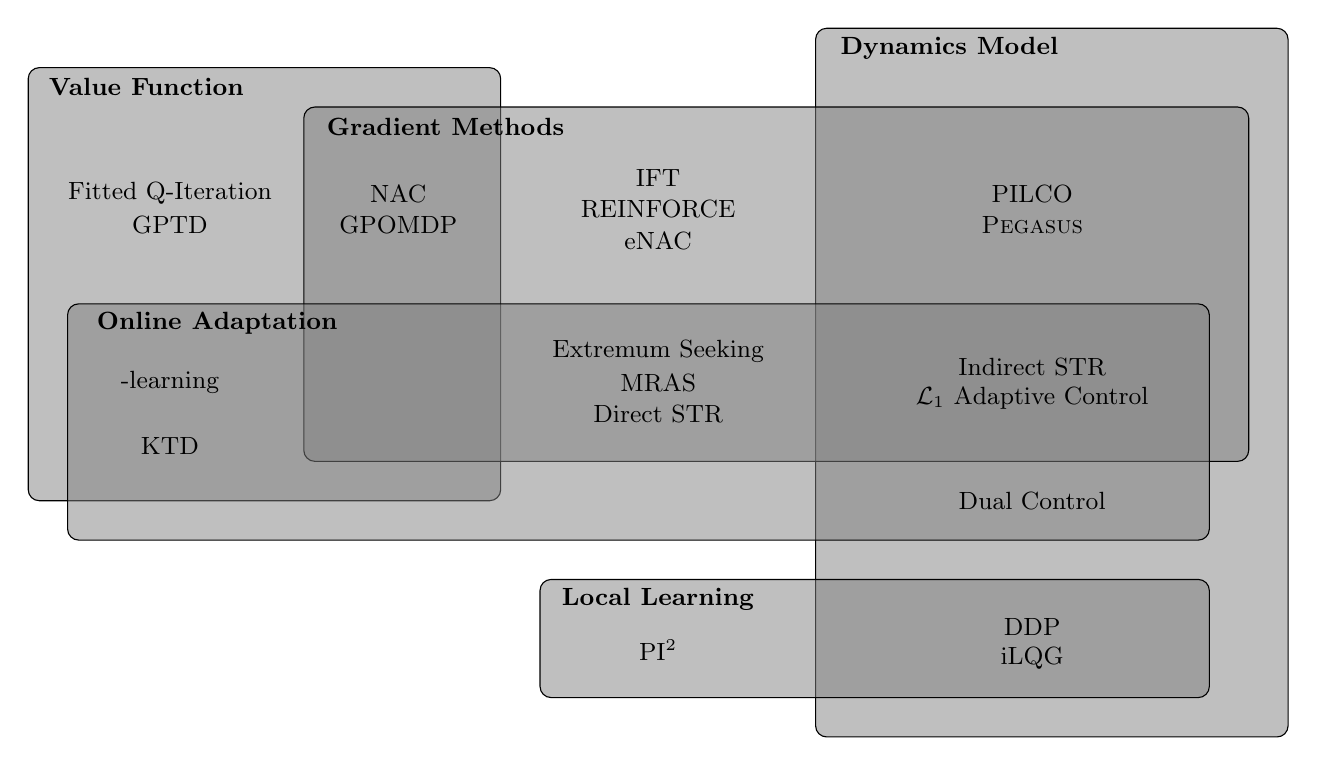
\begin{tikzpicture}
    \begin{scope}[fill opacity=0.5]
        \draw[rounded corners, fill=gray] (2,-0.5) rectangle (8,8.5);
        \draw[rounded corners, fill=gray] (-8,2.5) rectangle (-2,8);
        \draw[rounded corners, fill=gray] (-4.5,3) rectangle (7.5,7.5);
        \draw[rounded corners, fill=gray] (-7.5,2) rectangle (7,5);
        \draw[rounded corners, fill=gray] (-1.5,0) rectangle (7,1.5);
    \end{scope}
    
    \node at (3.7,8.25){{\small\textbf{Dynamics Model}}};
    \node at (-6.5,7.75){{\small\textbf{Value Function}}};
    \node at (-2.7,7.25){{\small\textbf{Gradient Methods}}};
    \node at (0,1.25){{\small\textbf{Local Learning}}};
    \node at (-5.6,4.75){{\small\textbf{Online Adaptation}}};
    
    \node at (-6.2,4){{\small \Q-learning}};
    \node at (-6.2,3.6){{\small \SARSA}};
    \node at (-6.2,3.2){{\small KTD}};
    \node at (-6.2,6.4){{\small Fitted Q-Iteration}};
    \node at (-6.2,6){{\small GPTD}};
    \node at (-3.3,6.4){{\small NAC}};
    \node at (-3.3,6){{\small GPOMDP}};
    \node at (4.75,6.4){{\small PILCO}};
    \node at (4.75,6){{\small \textsc{Pegasus}}};
    \node at (0,4.4){{\small Extremum Seeking}};
    \node at (0,4){{\small MRAS}};
    \node at (0,3.6){{\small Direct STR}};
    \node at (4.75,4.2){{\small Indirect STR}};
    \node at (4.75,3.8){{\small $\mathcal{L}_1$ Adaptive Control}};
    \node at (0,6.6){{\small IFT}};
    \node at (0,6.2){{\small REINFORCE}};
    \node at (0,5.8){{\small eNAC}};
    \node at (0,0.6){{\small PI$^2$}};
    \node at (4.75,0.9){{\small DDP}};
    \node at (4.75,0.5){{\small iLQG}};
    \node at (4.75,2.5){{\small Dual Control}};
\end{tikzpicture}
\caption{Summary of learning algorithms from adaptive control and reinforcement learning. }
\label{figs:venny}
\end{figure}

